\begin{abstract}
We study the least amplitude required to satisfy finitely many linear moment
conditions under a Lipschitz constraint. Starting from a sign certificate for the
unconstrained problem, we obtain a fourth-order expansion in the reciprocal slope
budget. Its coefficient contains a nonnegative quadratic correction caused by
the lower moment constraints. The result covers both finitely many switches on
a compact interval and countably many separated switches on the half-line, under
an explicit weighted summability condition. Examples show that the fourth-order
coefficient can have either sign, and that twice continuous differentiability
alone does not imply a fourth-order expansion. For a positive theta-kernel
family along a short, validated cusp branch, we give uniform, explicit
sixth-order error bounds. A weighted change of scale then proves strict ordering
of the actual optimal values for every pair of distinct branch parameters,
including arbitrarily close pairs. The numerical claims are accompanied by
interval certificates and reproducible checks. This preprint is prepared for
independent mathematical review; neither a formal verification nor an external
referee report is claimed.
\end{abstract}

\noindent\textbf{Keywords.} Moment constraints; Lipschitz optimization;
bounded Lipschitz norm; asymptotic expansion; computer-assisted proof;
theta kernel; cusp.

\section{Problem and contribution}
Let \(X\) be a compact interval or \([0,\infty)\), let
\(q_0,\ldots,q_m\) be real integrable functions, and let \(m\geq1\), \(f>0\).
For \(M>0\), define
\begin{equation}\label{eq:problem}
 \delta(M)=\inf\left\{\norm{g}_\infty:
 \Lip(g)\leq M,\quad
 \int_Xq_jg=0\ (0\leq j<m),\quad \int_Xq_mg=f\right\}.
\end{equation}
The functions \(g\) are real and Lipschitz; endpoint values are free.
Amplitude and slope are separate constraints. Put
\[
 q_b=q_m-\sum_{j<m}b_jq_j,\qquad
 H_b(a)=\sup_{\norm{s}_\infty\leq1,\ \Lip(s)\leq1/a}\int_Xq_bs.
\]
The latter is a one-dimensional bounded Lipschitz support problem, closely
related to the Kantorovich--Rubinstein and Fortet--Mourier frameworks
\cite{lellmann,hille2023,hille2024}. We do not claim a new dual norm or a new
principle of slope saturation.

Assume that a vector \(b^*\) gives the sign certificate
\begin{equation}\label{eq:signcertificate}
 q_*=q_{b^*},\qquad
 \int_Xq_j\sgn q_*=0\quad(j<m),\qquad D=\int_X|q_*|>0 .
\end{equation}
Then the problem without the Lipschitz constraint has value
\(\delta_0=f/D\). Indeed \(f=\int q_*g\leq D\norm{g}_\infty\),
and \(g=\delta_0\sgn q_*\) realizes equality in the measurable class.

Our main result identifies both coefficients in
\[
 \delta(M)=\delta_0+\frac{C_2}{M^2}+\frac{C_4}{M^4}+o(M^{-4})
 \qquad(M\longrightarrow\infty).
\]
The explicit fourth coefficient, the treatment of an infinite switch set, and
the application with uniform error and transport bounds are the contributions
for which this manuscript seeks review. We distinguish these claims from the
established optimization framework. An exhaustive priority claim is not made.

Section~\ref{sec:general} states and proves the general result.
Section~\ref{sec:examples} gives exact examples and a regularity obstruction.
Section~\ref{sec:theta} specializes it to a positive integral family and states
the computer-assisted bounds. Section~\ref{sec:transport} proves a general
transport comparison and its strict-order consequence. The appendices explain
the effective estimates and the interface between the analytic proof and the
computational evidence.

\section{Fourth-order value asymptotics}\label{sec:general}
At each simple zero \(z_k\) of \(q_*\), write
\[
 Q_k=(q_j(z_k))_{j<m},\quad r_k=q_*'(z_k),\quad
 t_k=q_*''(z_k),\quad u_k=q_*'''(z_k),\quad
 \gamma_k=|r_k|,\quad \sigma_k=\sgn r_k.
\]
Define the following quantities whenever their series converge:
\begin{align}
 \Gamma&=\sum_k\gamma_k,&
 G&=2\sum_k\frac{Q_kQ_k^{\mathsf T}}{\gamma_k},\label{eq:GB}\\
 B_j&=\frac13\sum_k\sigma_k
       \left(\frac{q_j(z_k)t_k}{r_k}-q_j'(z_k)\right),&
 v&=G^{-1}B,\nonumber\\
 R&=\sum_k\left(\frac{t_k^2}{36\gamma_k}
                    -\frac{\sigma_ku_k}{60}\right),&
 P&=\frac12B^{\mathsf T}G^{-1}B,\qquad \Xi=R-P.\label{eq:RP}
\end{align}
Here \(G\) is an \(m\)-by-\(m\) matrix and \(B,v\in\R^m\).

\subsection{Countably many switches}
We impose the following hypotheses on \(X=[0,\infty)\).
\begin{enumerate}[label=(H\arabic*),leftmargin=*]
\item The functions \(q_j\) are in \(L^1(X)\) and are locally \(C^3\).
The sign certificate \eqref{eq:signcertificate} holds, \(q_*(0)\ne0\), and
the positive zeros \(z_k\) tend to infinity with positive minimum separation.
\item There are disjoint neighborhoods \(N_k=[z_k-\rho,z_k+\rho]\subset(0,\infty)\),
with a common \(\rho>0\), and a bounded open neighborhood \(U\) of \(b^*\).
For every \(b\in U\), \(q_b\) has exactly one zero \(z_k(b)\) in each \(N_k\)
and no other zeros. The orientations remain \(\sigma_k\).
The functions \(z_k(b)\) are \(C^1\), have a common Lipschitz constant, and
\(|z_k(b)-z_k|<\rho/4\).
\item There are \(L_k>0\) such that
\(|q_b(x)|\geq L_k|x-z_k(b)|\) on \(N_k\) for all \(b\in U\).
Set
\[
 E_k=\sum_{j=0}^m\sum_{\ell=0}^3\sup_{N_k}|q_j^{(\ell)}|,
 \quad C_U=1+\sup_{b\in U}\sum_{j<m}|b_j|,
 \quad K_k=\frac{C_UE_k}{6L_k}.
\]
The weighted condition is
\begin{equation}\label{eq:weighted}
 \sum_kE_k(1+K_k)^2<\infty.
\end{equation}
The sequence \(K_k\) need not be bounded.
\item Some \(m\) vectors among the \(Q_k\) are linearly independent.
\end{enumerate}

\begin{theorem}\label{thm:infinite}
Under {\rm(H1)--(H4)}, all the series in \eqref{eq:GB}--\eqref{eq:RP}
converge absolutely, \(G\) is positive definite, and \eqref{eq:problem}
has an optimizer for all sufficiently large \(M\). Moreover,
\begin{align}
 \delta(M)&=\delta_0+C_2M^{-2}+C_4M^{-4}+o(M^{-4}),\label{eq:expansion}\\
 C_2&=\frac{\delta_0^3\Gamma}{3D},&
 C_4&=\delta_0^5\left(\frac{\Gamma^2}{3D^2}-\frac{R}{D}
                          +\frac{P}{D}\right).\label{eq:coefficients}
\end{align}
The term \(P\) is nonnegative and is unchanged by any invertible linear
change of basis of the lower moment functions \(q_0,\ldots,q_{m-1}\).
\end{theorem}

We give the proof, including the tail and exact-feasibility steps.
For an average over \([-1,1]\), write
\(\mathbb E h(y)=\frac12\int_{-1}^1h(y)\dd y\).

\begin{lemma}[Balanced ramps]\label{lem:ramps}
For all \(b\in U\) sufficiently close to \(b^*\) and all sufficiently small
\(a>0\), there is a unique center \(c_k\in(z_k(b)-a,z_k(b)+a)\) satisfying
\begin{equation}\label{eq:balance}
 \mathbb E q_b(c_k+ay)=0.
\end{equation}
Its displacement satisfies
\[
 |c_k-z_k(b)|\leq\min\{a,K_ka^2\}.
\]
The function equal to \(\sgn q_b\) outside the ramp intervals and equal
to \(\sigma_k(x-c_k)/a\) on \([c_k-a,c_k+a]\) maximizes \(H_b(a)\).
\end{lemma}
\begin{proof}
At \(c=z_k(b)-a\) and \(c=z_k(b)+a\), the averaged function has opposite
signs. Between them its derivative is
\([q_b(c+a)-q_b(c-a)]/(2a)\), of strict sign \(\sigma_k\).
Taylor's theorem gives
\(|q_b(c)-\mathbb E q_b(c+ay)|\leq C_UE_ka^2/6\).
The crossing bound then proves the displacement estimate.

On a balanced interval \([\ell,r]\), put
\(J(x)=\int_\ell^xq_b(t)\dd t\).
There is just one change of sign of \(q_b\), and
\(J(\ell)=J(r)=0\), \(\sigma_kJ(x)<0\) inside.
For any competitor \(s\), integration by parts gives
\[
 \int_\ell^rq_b(s-s_a)
   =-\int_\ell^rJ(x)(s'(x)-\sigma_k/a)\dd x\leq0.
\]
Outside these intervals, \(s_a=\sgn q_b\) maximizes the integrand
pointwise. The intervals are disjoint for small \(a\).
The infinite sum is justified by the integrable bound \(2|q_b|\).
\end{proof}

\begin{proof}[Proof of Theorem~\ref{thm:infinite}]
\emph{Convergence and coefficients.}
Differentiating the zero equation gives
\(\partial_{b_j}z_k=q_j(z_k)/r_k\).
The common root Lipschitz bound in (H2) therefore bounds \(Q_k/r_k\).
Also \(|t_k/r_k|\leq6K_k\).
These estimates and \eqref{eq:weighted} imply absolute convergence of
\(\Gamma,G,B,R\). Condition (H4) makes \(G\) positive definite.

Choose the trial multiplier \(b(a)=b^*+va^2\) and its balanced ramp
profile \(s_a\). This trial multiplier is not asserted to solve the exact
dual optimization problem. Define
\begin{equation}\label{eq:kappa}
 \kappa_k=\frac{Q_k^{\mathsf T}v-t_k/6}{r_k}.
\end{equation}
Implicit differentiation of the zero equation and
\eqref{eq:balance}, for each fixed \(k\), give
\[
 \Delta_k:=c_k-z_k=\kappa_ka^2+o(a^2).
\]
Uniformly in \(k\), for a fixed constant \(C\),
\begin{equation}\label{eq:displacements}
 |\Delta_k|\leq a+C\norm{v}a^2\leq2a,\qquad
 |\Delta_k|/a^2\leq K_k+C\norm{v}.
\end{equation}
The first estimate and the second serve different purposes; we do not
replace them by a false uniform bound on \(\kappa_k\).

\emph{Summed moment expansions.}
For \(H_j(t)=\int_t^\infty q_j(x)\dd x\), the moment change at a switch is
\[
 2\sigma_k\{\mathbb E H_j(z_k+\Delta_k+ay)-H_j(z_k)\}.
\]
Only these differences are summed; separate sums of the \(H_j(z_k)\)
are unnecessary. If \(h=\Delta_k+ay\), then
\[
 \mathbb E h=\Delta_k,\quad
 \mathbb E h^2=\Delta_k^2+a^2/3,\quad
 \mathbb E h^3=\Delta_k^3+\Delta_ka^2,\quad
 \mathbb E h^4=\Delta_k^4+2\Delta_k^2a^2+a^4/5 .
\]
Taylor expansion and \eqref{eq:displacements} now yield
\begin{align}
 \int q_js_a&=a^2(B-Gv)_j+o(a^2)=o(a^2)\quad(j<m),\label{eq:defect}\\
 \int q_*s_a&=D-\frac{\Gamma a^2}{3}
 -a^4\sum_k\sigma_k
 \left(r_k\kappa_k^2+\frac{t_k\kappa_k}{3}+\frac{u_k}{60}\right)
 +o(a^4).\label{eq:targetexp}
\end{align}
Here the normalized lower moment terms and the target terms are dominated
by a constant times \(E_k(1+K_k)^2\).
For example, \(r_k\Delta_k^2/a^4\) uses the second bound in
\eqref{eq:displacements}; terms of degree at least four use
\(|\Delta_k|\leq2a\) as well. The Taylor remainder divided by \(a^4\)
tends to zero for each fixed \(k\), by continuity of \(q_*'''\), and has
the same summable majorant. Dominated convergence proves both displayed
expansions.

Completing the square with \eqref{eq:kappa} gives
\[
 -\sum_k\sigma_k
 (r_k\kappa_k^2+t_k\kappa_k/3+u_k/60)
   =R-\tfrac12v^{\mathsf T}Gv=\Xi .
\]
Since \(q_{b(a)}=q_*-a^2\sum v_jq_j\),
\eqref{eq:defect} also gives the support expansion
\begin{equation}\label{eq:supportexp}
 H_{b(a)}(a)=D-\Gamma a^2/3+\Xi a^4+o(a^4).
\end{equation}
For a general trial vector \(v\), its fourth coefficient would be
\(R+\tfrac12v^{\mathsf T}Gv-B^{\mathsf T}v\);
its minimum occurs at \(G^{-1}B\).

\emph{Exact moment repair.}
Select the \(m\) independent switches from (H4), and move only their
centers by a vector \(e\). At \(a=0,e=0\), the derivative of the lower
moment map has columns \(-2\sigma_kQ_k\), so it is invertible.
For small \(a\) this derivative remains uniformly close to that invertible
matrix. A contraction with that matrix as preconditioner, on a ball of
radius a fixed multiple of the defect in \eqref{eq:defect}, gives a
continuous solution \(e(a)=o(a^2)\).
Indeed its forcing is \(o(a^2)\), and its derivative norm can be made
less than \(1/2\), so that this ball maps into itself.
Ramp intervals remain disjoint and the amplitude and slope bounds are
unchanged. The derivative of the \(q_*\) moment with respect to each
selected center is \(O(a^2)\), while its second derivative is bounded.
Consequently the repair changes that moment by
\(O(a^2|e|+|e|^2)=o(a^4)\).
The repaired profile \(\widetilde s_a\) therefore has exact lower
moments and
\begin{equation}\label{eq:primalexp}
 S(a):=\int q_m\widetilde s_a
      =D-\Gamma a^2/3+\Xi a^4+o(a^4).
\end{equation}

Put \(A(a)=f/S(a)\) and \(M(a)=A(a)/a\).
The feasible function \(A(a)\widetilde s_a\) has amplitude \(A(a)\)
and slope at most \(M(a)\). Both functions are continuous for small
positive \(a\), \(A(a)\to\delta_0\), and \(M(a)\to\infty\).
The image of this interval under \(M(a)\) is an interval unbounded
above, hence contains all sufficiently large budgets. No monotonicity
of this parametrization is needed.

\emph{Attainment and matching lower bound.}
For a fixed sufficiently large \(M\), a minimizing sequence is uniformly
bounded and equicontinuous. A diagonal Arzel\`a--Ascoli argument gives a
locally uniform limit. Dominated convergence against each \(q_j\in L^1\)
preserves the moments, and the norm and Lipschitz bounds pass to the
limit. Thus the optimum is attained.

For any feasible amplitude \(A\), use
\(a=A/M\), \(s=g/A\), and the trial multiplier at that \(a\). Then
\[
 f=\int q_{b(a)}g\leq A H_{b(a)}(a).
\]
The preceding feasible upper bound and \(\delta(M)\geq\delta_0\)
show that the minimizing amplitude tends to \(\delta_0\).
The support and primal expansions therefore have matching scalar
inversions. Explicitly, with
\(t=\Gamma/(3D)\), \(e=\Xi/D\), the equation to this order is
\[
 A\{1-t(A/M)^2+e(A/M)^4+o(M^{-4})\}=\delta_0 .
\]
Its increasing polynomial part has derivative bounded away from zero
near \(\delta_0\). The remainder is uniform for \(A\) in a compact
neighborhood of \(\delta_0\). Substitution yields
\[
 A=\delta_0+t\delta_0^3M^{-2}
                   +(3t^2-e)\delta_0^5M^{-4}+o(M^{-4}),
\]
which proves \eqref{eq:coefficients}. In particular the factor \(3\)
accounts for the dependence \(a=A/M\).
Finally, a lower-moment basis change \(Q\mapsto LQ\) gives
\(G\mapsto LGL^{\mathsf T}\), \(B\mapsto LB\), and leaves \(P\) unchanged.
\end{proof}

\subsection{Finite switch sets and the role of the constraints}
\begin{proposition}\label{prop:finite}
On a compact interval, suppose the \(q_j\) are \(C^2\), that
\eqref{eq:signcertificate} holds, that all zeros of \(q_*\) are finitely
many simple interior zeros, with no endpoint zeros, and that the \(Q_k\)
span \(\R^m\). For all sufficiently large \(M\), the optimum in
\eqref{eq:problem} is unique and consists of constant plateaus joined by
linear ramps. Its value satisfies
\[
 \delta(M)=\delta_0+\frac{\delta_0^3\Gamma}{3D}M^{-2}+o(M^{-3}).
\]
If \(q_*\) is \(C^3\) near the zeros, the full expansion
\eqref{eq:expansion}--\eqref{eq:coefficients} holds with finite sums.
\end{proposition}
\begin{proof}
Root separation and sign persistence are automatic on a compact interval
after shrinking the neighborhood of \(b^*\).
The balance equations define centers \(c_k(a,b)\).
At \(a=0\) the lower-moment map of their ramp profile has \(b\)-derivative
\(-G\). Expressing its local contributions as averages of primitives
shows that this map is \(C^2\), including at \(a=0\).
The implicit function theorem supplies an even \(C^2\) multiplier \(b(a)\)
which makes all lower moments exactly zero.
Thus \(b(a)=b^*+va^2+o(a^2)\), with \(v\) as above.

Lemma~\ref{lem:ramps} proves exact support optimality.
Equality forces \(s=\sgn q_b\) on every plateau and
\(s'=\sigma_k/a\) almost everywhere in every ramp, because
\(\sigma_kJ<0\) there. Continuity fixes all endpoint values.
The support maximizer, and hence the constrained optimizer at the
resulting budget, is unique.
The target satisfies \(S(a)=D-\Gamma a^2/3+o(a^3)\) under \(C^2\)
regularity; its derivative is \(O(a)\).
Hence \(M(a)=f/(aS(a))\) has negative derivative for small \(a>0\)
and covers all sufficiently large budgets. The scalar inversion gives
the stated second-order result. If \(q_*\) is \(C^3\) near the switches,
the finite version of \eqref{eq:targetexp} gives the fourth coefficient.
\end{proof}

\begin{remark}
The sign of \(C_4\) is not fixed by positivity of an underlying weight.
The nonnegative quantity \(P\) has a more specific interpretation.
For the fixed residual \(q_*\), the unconstrained ramp support has
fourth coefficient \(R\); imposing the lower moments gives \(\Xi=R-P\).
Thus the loss at this order is \(Pa^4\).
This does not compare the original \(q_m\) problem with a different
problem in which all lower constraints have simply been deleted.
\end{remark}

\section{Exact examples and a regularity obstruction}\label{sec:examples}
These examples have \(X=[-1,1]\), \(m=1\), \(q_0=1\), and \(b^*=0\).
They permit direct integration, independently of the coefficient formulas.

\subsection{An asymmetric two-switch example}
Let
\[
 q_1(x)=(x^2-\tfrac14)(1+\beta x),\qquad |\beta|<1,\qquad f=\tfrac18 .
\]
The zeros are \(\pm1/2\), and the sign has zero mean.
For small \(a\), exact mean balance puts the two centers at
\(c_\pm=d\pm1/2\). Their individual balance equations coincide:
\[
 2d+3\beta d^2+\beta a^2=0 .
\]
The solution near zero is
\(d=-\beta a^2/2-3\beta^3a^4/8+O(a^6)\).
Integration of the resulting profile gives
\[
 S(a)=\tfrac12-\tfrac23a^2+\tfrac{\beta^2}{2}a^4+O(a^6).
\]
In particular,
\begin{equation}\label{eq:exampleone}
 \delta_0=\tfrac14,\qquad C_2=\tfrac1{48},\qquad
 C_4=\frac{16/3-\beta^2}{1024}.
\end{equation}
As an exact arithmetic check, for \(\beta=1/4\),
\[
 G=\frac{256}{63},\quad B=\frac{244}{189},\quad
 R=\frac{134}{567},\quad P=\frac{3721}{18144},\quad
 \Xi=\frac1{32},\quad C_4=\frac{253}{49152}.
\]
The cancellation producing \(\Xi\) is substantial enough that retaining
the moment correction matters.

\subsection{A negative fourth coefficient}
Let \(q_1(x)=x-3x^3+9x^5\) and \(f=5/8\).
Since \(q_1=x\{(3x^2-1/2)^2+3/4\}\), there is a single simple switch
at zero. Odd symmetry gives the balanced center exactly.
The supported moment is
\[
 S(a)=\tfrac52-\tfrac13a^2+\tfrac3{10}a^4-\tfrac37a^6.
\]
Inverting with \(a=A/M\) gives
\begin{equation}\label{eq:examplenegative}
 \delta(M)=\tfrac14+\frac1{480M^2}
                        -\frac1{15360M^4}+O(M^{-6}).
\end{equation}
The underlying weight here is the positive constant \(1\), so it cannot
enforce positivity of \(C_4\).

\subsection{Why twice continuous differentiability is insufficient}
Let \(q_1(x)=x+\sgn(x)|x|^{5/2}\) and \(f=11/28\).
This function is \(C^2\), with a simple zero at zero, but is not \(C^3\).
The exact ramp moment is
\[
 S(a)=\frac{11}{7}-\frac{a^2}{3}-\frac{8a^{7/2}}{63}.
\]
Consequently,
\begin{equation}\label{eq:regularityexample}
 \delta(M)=\tfrac14+\frac7{2112M^2}
                         +\frac1{6336M^{7/2}}+O(M^{-4}).
\end{equation}
Thus a finite coefficient in a remainder of the form
\(C_4M^{-4}+o(M^{-4})\) after the second-order term does not exist.
This is consistent with the \(o(M^{-3})\) conclusion under \(C^2\).

\begin{figure}[tb]
 \centering
 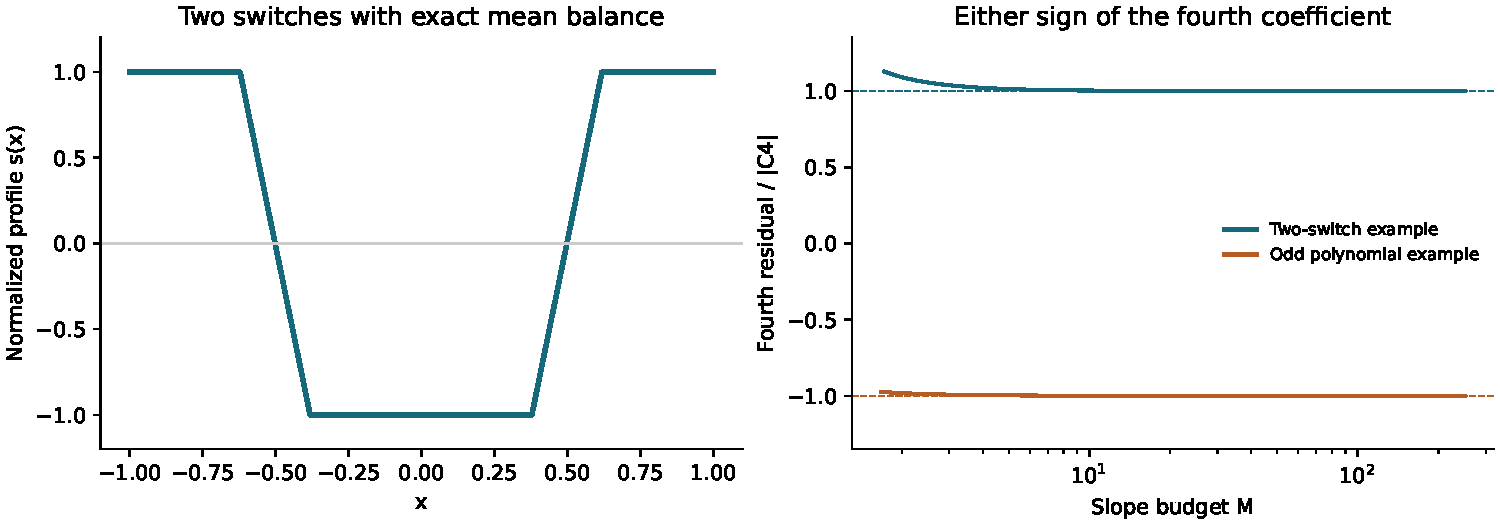
\includegraphics[width=.96\linewidth]{figures/examples.pdf}
 \caption{Left: the unique normalized optimizer in the two-switch
 example with \(\beta=1/4\) at ramp half-width \(a=0.12\), computed
 from its exact balance equation. Right: the scaled residual
 \(M^4(\delta(M)-\delta_0-C_2/M^2)/|C_4|\) for the first two examples,
 with the analytic limits \(+1\) and \(-1\) as dashed lines.
 The curves are high-precision evaluations of their explicit scalar
 equations, not interval certificates.}
 \label{fig:examples}
\end{figure}

\section{A positive theta-kernel family}\label{sec:theta}
Define, for \(u\geq0\),
\begin{align}
 \Phi(u)&=\sum_{n\geq1}\pi n^2e^{5u}
       (2\pi n^2e^{4u}-3)\exp(-\pi n^2e^{4u}),\label{eq:theta}\\
 F(t;\lambda,\mu,\nu)&=\int_0^\infty
       \Phi(u)e^{\lambda u^2+\mu u^4+\nu u^6}\cos(2tu)\dd u .
                                                        \label{eq:F}
\end{align}
Every summand of \(\Phi\) is positive on this domain.
Double exponential decay permits parameter differentiation on compact
sets, including complex parameter sets.
Write \(D_j=\partial_t^jF\). Then
\begin{equation}\label{eq:momentdictionary}
 \partial_\lambda D_j=-D_{j+2}/4,\qquad
 \partial_\mu D_j=D_{j+4}/16,\qquad
 \partial_\nu D_j=-D_{j+6}/64 .
\end{equation}

\subsection{The cusp branch and the design problem}
A validated zero of \((D_0,D_1,D_2)\) at \(\nu=0\) has the rounded
location
\[
 (t,\lambda,\mu)\simeq
 (41.4003413586842508894,\,
  -3.64569206160491909881,\,
   8.33512049891860723771).
\]
These displayed coordinates are explanatory approximations; the
companion certificate specifies the actual enclosing box.
At that zero,
\begin{align*}
 3.33563055\cdot10^{-13}&<D_3<3.33563057\cdot10^{-13},\\
 -9.71679534\cdot10^{-13}&<D_4<-9.71679532\cdot10^{-13}.
\end{align*}
In particular the control determinant for the equations \(D_0=D_1=0\)
is \(D_3D_4/64\ne0\), and \(D_3\ne0\) gives the usual local cusp
geometry of the zero set of \(F\). A computer-assisted continuation
defines a single analytic branch
\[
 Q(\nu)=(\tau(\nu),\lambda(\nu),\mu(\nu)),\qquad
 \nu\in I=[-1/64,0].
\]
Shared parameter faces are joined by root containment in the next
uniqueness box, not merely by overlap of the surrounding boxes.
The validated continuation methods are used to establish the particular
branch and bounds here; cusp validation as a general method is established
in the literature \cite{lessard}.

Differentiating the three cusp equations gives the useful identities
\begin{align}
 \mu'&=D_6/(4D_4),&
 \lambda'&=(4D_5\mu'-D_7)/(16D_3),\nonumber\\
 \tau'&=(D_8/64+D_4\lambda'/4-D_6\mu'/16)/D_3 .\label{eq:velocity}
\end{align}
Set
\[
 w_\nu(u)=\Phi(u)e^{\lambda(\nu)u^2+\mu(\nu)u^4+\nu u^6},\qquad
 p_{j,\nu}(u)=(2u)^j\cos(2\tau(\nu)u+j\pi/2),
\]
and let \(q_{j,\nu}=w_\nu p_{j,\nu}\), \(0\leq j\leq3\).
In \eqref{eq:problem} take \(m=3\) and
\(f_\nu=D_3(Q(\nu),\nu)>0\), and denote its value by \(\delta_\nu(M)\).
All coefficients in Section~\ref{sec:general} now depend on \(\nu\).

If \(g\) is feasible, multiplying the kernel by \(1-g\) makes the
first four \(t\)-derivatives, of orders \(0,1,2,3\), vanish at the
prescribed point. If \(\norm{g}_\infty<1\), the modified kernel is still
positive. The size \(\delta_\nu(M)\) is therefore the least amplitude of
such a constrained change, with its roughness controlled by \(M\).
This interpretation concerns a separate profile for each \(\nu\).

\begin{theorem}[Theta value enclosure]\label{thm:theta}
For every \(\nu\in I\), the sign certificate and hypotheses of
Theorem~\ref{thm:infinite} hold for the kernels just defined.
For every \(M\geq M_0=2\cdot10^{-5}\), the optimum is attained and
\[
 9.17\cdot10^{-10}<\delta_\nu(M)<9.181\cdot10^{-10}<1 .
\]
With \(P_{4,\nu}(M)=\delta_{0,\nu}+C_{2,\nu}M^{-2}+C_{4,\nu}M^{-4}\),
\begin{equation}\label{eq:thetaerror}
 -\frac{1.02\cdot10^{-53}}{M^6}
 <\delta_\nu(M)-P_{4,\nu}(M)
 <\frac{1.64\cdot10^{-53}}{M^6}.
\end{equation}
Furthermore, throughout \(I\),
\begin{align}
 2.48374879\cdot10^{-39}&<C_{4,\nu}<2.49203006\cdot10^{-39},
                                                        \label{eq:C4range}\\
 2.7\cdot10^{-11}&<\delta_{0,\nu}'<3.0\cdot10^{-11},\nonumber\\
 7.4\cdot10^{-26}&<C_{2,\nu}'<8.7\cdot10^{-26},\nonumber\\
 1.9\cdot10^{-40}&<C_{4,\nu}'<5.3\cdot10^{-40}.\label{eq:coefficientmotion}
\end{align}
\end{theorem}

\begin{proof}[Proof structure and computational evidence]
The branch construction, sign equations, invertible moment Jacobian,
simple residual zeros, and derivative bounds are established on
32 closed driver cells
\[
 I_i=[-(i+1)/2048,-i/2048],\qquad 0\leq i<32.
\]
The moment Jacobian is \(-G\); its nonsingularity and the convexity of
\(\int|q_b|\) identify the local dual solution as the unique global
minimizer. For clarity, a second minimizer would make the objective
constant on their joining segment, contradicting its positive
definite Hessian near the certified minimizer.

The residual without its positive weight has the form
\begin{equation}\label{eq:rawresidual}
 r_b(u)=(8u^3+2b_1u)\sin(2\tau u)
                  +(4b_2u^2-b_0)\cos(2\tau u).
\end{equation}
On \([0,1]\), the evidence isolates 28 simple zeros and covers their
complement by sign enclosures. On \(u\geq1\), put
\(T=( (8u^3+2b_1u)^2+(4b_2u^2-b_0)^2)^{1/2}\) and
\(\phi=2\tau u+\arctan((4b_2u^2-b_0)/(8u^3+2b_1u))\).
The uniform bounds
\[
 T>7u^3,\quad |T'|<25u^2,\quad 81<\phi'<85
\]
give separated, simple zeros, with spacing greater than \(3/85\) and
\(|r_b'|>567u^3\) at each zero.
They also bound root motion with \(b\), since
\(|\partial_{b_j}z|\leq1/(81z)\) for the tail zeros.

The weight decay verifies the stronger, weighted hypothesis
\eqref{eq:weighted}, rather than only unweighted convergence.
For \(H=1/64\) and \(\rho\leq1/1000\), suitable uniform constants give
\begin{align*}
 E_k&\leq C(1+z_k+\rho)^{18}
 e^{21(z_k+\rho)+9(z_k+\rho)^4-\pi e^{4(z_k-\rho)}},\\
 L_k&=e^{-4(z_k+\rho)^2-H(z_k+\rho)^6-\pi e^{4(z_k+\rho)}}.
\end{align*}
The ratio \(E_k^3/L_k^2\) is bounded by a polynomial times
\[
 \exp\{63(z_k+\rho)+27(z_k+\rho)^4+8(z_k+\rho)^2
       +2H(z_k+\rho)^6-\pi c_\rho e^{4z_k}\},
 \quad c_\rho=3e^{-4\rho}-2e^{4\rho}>0.97 .
\]
The separated zeros and this double exponential decay prove
\eqref{eq:weighted}. Finite initial neighborhoods are covered directly.
Theorem~\ref{thm:infinite} now applies.

The explicit remainder requires additional estimates and does not
follow just from that theorem. Appendix~\ref{app:effective} constructs
finite ramp profiles with exact moments and an accompanying support
bound, uniformly on all 32 cells. Scalar comparison, without continuity
of the number of active ramps, proves \eqref{eq:thetaerror} and
feasibility for every stated \(M\).
Differentiated coefficient identities and interval enclosures give
\eqref{eq:C4range}--\eqref{eq:coefficientmotion}.
The exact input-output map and replay commands appear in
Appendix~\ref{app:evidence}; those finite computations are part of this
computer-assisted theorem.
\end{proof}

At \(M=M_0\), the absolute error in \eqref{eq:thetaerror} lies between
\(-1.59375\cdot10^{-25}\) and \(2.5625\cdot10^{-25}\).
These figures measure the truncation error once the coefficients are
known; rounding the coefficients separately introduces additional
error. In particular the broad uniform ranges above are not substitutes
for pointwise coefficient enclosures.

\section{Transport and strict ordering of the optimal value}\label{sec:transport}
The coefficient derivatives in \eqref{eq:coefficientmotion} and a uniform
remainder suffice to compare well-separated parameters. They do not by
themselves compare the actual values at arbitrarily close parameters.
We use a change of scale which preserves all the moment equations.
Weighted composition operators on Lipschitz spaces are an established
framework \cite{abbar}; the result below is a sufficient differential
condition adapted to these moments and to a specified amplitude-to-slope
ratio.

\begin{theorem}[Moment-preserving transport]\label{thm:transport}
Suppose \(w_\nu(u)>0\) is \(C^2\) in \(u\), is \(C^1\) in \(\nu\),
and has continuous mixed derivative \(\partial_u\partial_\nu\log w_\nu\).
Suppose \(f_\nu>0\) and \(\tau(\nu)>0\) are \(C^1\).
Assume that the following kernels are integrable on the half-line:
\[
 q_{j,\nu}(u)=w_\nu(u)(2u)^j
                 \cos(2\tau(\nu)u+j\pi/2),\quad 0\leq j\leq m .
\]
Let \(\kappa=-\tau'/\tau\geq0\), \(L_\nu=\partial_u\log w_\nu\), and
\[
 r_\nu(u)=-f_\nu'/f_\nu+(m+1)\kappa
               +\partial_\nu\log w_\nu(u)+\kappa uL_\nu(u).
\]
If for constants \(a_0,c>0\)
\begin{equation}\label{eq:transportcriterion}
 r_\nu+\kappa+a_0|\partial_ur_\nu|\leq-c
\end{equation}
throughout a parameter interval and the whole half-line, then for
\(\nu_1<\nu_2\), \(d=\nu_2-\nu_1\), \(\eta=\tau(\nu_1)/\tau(\nu_2)\),
the transformation
\begin{equation}\label{eq:transportmap}
 (\mathcal T g)(u)=T(u)g(\eta u),\qquad
 T(u)=\frac{f_{\nu_1}}{f_{\nu_2}}\eta^{m+1}
                 \frac{w_{\nu_2}(\eta u)}{w_{\nu_1}(u)}
\end{equation}
preserves feasibility of the moment equations from \(\nu_2\) to \(\nu_1\).
If \(\norm{g}_\infty\leq a_0M\), \(\Lip(g)\leq M\), then
\[
 \norm{\mathcal T g}_\infty\leq e^{-cd}\eta^{-1}\norm{g}_\infty,
 \qquad \Lip(\mathcal T g)\leq e^{-cd}M .
\]
Consequently, whenever the optimum at \(\nu_2\) is attained with
amplitude at most \(a_0M\),
\begin{equation}\label{eq:order}
 \delta_{\nu_2}(M)\geq\eta e^{cd}\delta_{\nu_1}(M).
\end{equation}
\end{theorem}
\begin{proof}
Substitution \(x=\eta u\) and
\(p_{j,\nu_2}(\eta u)=\eta^jp_{j,\nu_1}(u)\) give the exact identity
\[
 \int q_{j,\nu_1}\mathcal T g
   =\frac{f_{\nu_1}}{f_{\nu_2}}\eta^{m-j}\int q_{j,\nu_2}g .
\]
This proves all moments, including the target at \(j=m\).

For the norm estimate, set \(\nu(t)=\nu_2-t\) and
\(\eta(t)=\tau(\nu(t))/\tau(\nu_2)\), and use \eqref{eq:transportmap}
with this moving first endpoint. Define
\(\mathcal D=\partial_t-\kappa u\partial_u\).
Direct logarithmic differentiation gives
\[
 \mathcal DT=rT,\qquad \eta'=\kappa\eta,\qquad
 \mathcal D(T_u)=(r+\kappa)T_u+r_uT .
\]
The positive commutator term \(+\kappa T_u\) is essential.
Since \(\eta\geq1\), \(T>0\), the quantity
\(W=\eta T+a_0|T_u|\) satisfies \(T\leq W\), and, along each
characteristic,
\[
 \mathcal DW\leq(r+\kappa)W+a_0|r_u|T\leq-cW .
\]
The inequality for the absolute value is valid almost everywhere;
alternatively it follows by regularization. Initially \(T=1,T_u=0\),
so \(W(0,u)=1\). Every finite endpoint characteristic has a finite
initial point. Thus no uniform boundedness of \(r\) at infinity is
needed, and
\[
 \eta T+a_0|T_u|\leq e^{-ct},\qquad T\leq e^{-ct}/\eta .
\]
The product and chain rules for Lipschitz functions prove the two norm
bounds. Applying them to an optimizer at \(\nu_2\) provides a feasible
competitor at \(\nu_1\) and proves \eqref{eq:order}.
\end{proof}

\begin{corollary}[Strict order on the theta branch]\label{cor:thetaorder}
For the family in Section~\ref{sec:theta}, for every \(M\geq2\cdot10^{-5}\)
and every \(-1/64\leq\nu_1<\nu_2\leq0\),
\begin{align}
 \delta_{\nu_2}(M)
 &\geq\frac{\tau(\nu_1)}{\tau(\nu_2)}
          e^{(\nu_2-\nu_1)/50}\delta_{\nu_1}(M)
  >\delta_{\nu_1}(M),\label{eq:thetaorder}\\
 \log\delta_{\nu_2}(M)-\log\delta_{\nu_1}(M)
 &>0.02259(\nu_2-\nu_1),\nonumber\\
 \delta_{\nu_2}(M)-\delta_{\nu_1}(M)
 &>2.07\cdot10^{-11}(\nu_2-\nu_1).\label{eq:linearorder}
\end{align}
These inequalities do not require differentiability or uniqueness of
the finite-budget optimizer.
\end{corollary}
\begin{proof}
The validated branch bounds include
\[
 .00259<\kappa<.00260,\quad .0437<f_\nu'/f_\nu<.0451,
 \quad .3260<\lambda'<.3264,\quad .2939<\mu'<.2942 .
\]
With \(a_0=2^{-14}\), Appendix~\ref{app:transport} proves
\eqref{eq:transportcriterion} with \(c=1/50\) on the whole half-line.
Theorem~\ref{thm:theta} gives
\(\delta_\nu(M)/M<9.181\cdot10^{-10}/(2\cdot10^{-5})<a_0\),
so Theorem~\ref{thm:transport} applies. Integrating the strict lower
bound for \(\kappa\) proves the logarithmic bound.
Finally \(e^x-1\geq x\) and
\(9.17\cdot10^{-10}\cdot.02259>2.07\cdot10^{-11}\)
give \eqref{eq:linearorder}.
\end{proof}

For a fixed nonzero separation, the coefficient bounds can give a sharper
two-sided estimate. Integrating \eqref{eq:coefficientmotion} and subtracting
the two errors in \eqref{eq:thetaerror} gives, with \(d=\nu_2-\nu_1\),
\[
 \mathcal L(M)d-\frac{2.66\cdot10^{-53}}{M^6}
 <\delta_{\nu_2}(M)-\delta_{\nu_1}(M)
 <\mathcal U(M)d+\frac{2.66\cdot10^{-53}}{M^6},
\]
where
\begin{align*}
 \mathcal L(M)&=2.7\cdot10^{-11}+7.4\cdot10^{-26}M^{-2}
                              +1.9\cdot10^{-40}M^{-4},\\
 \mathcal U(M)&=3.0\cdot10^{-11}+8.7\cdot10^{-26}M^{-2}
                              +5.3\cdot10^{-40}M^{-4}.
\end{align*}
The transport estimate remains strictly positive however small \(d>0\)
is; the fixed error allowance in the two-sided estimate cannot do this.

\begin{figure}[tb]
 \centering
 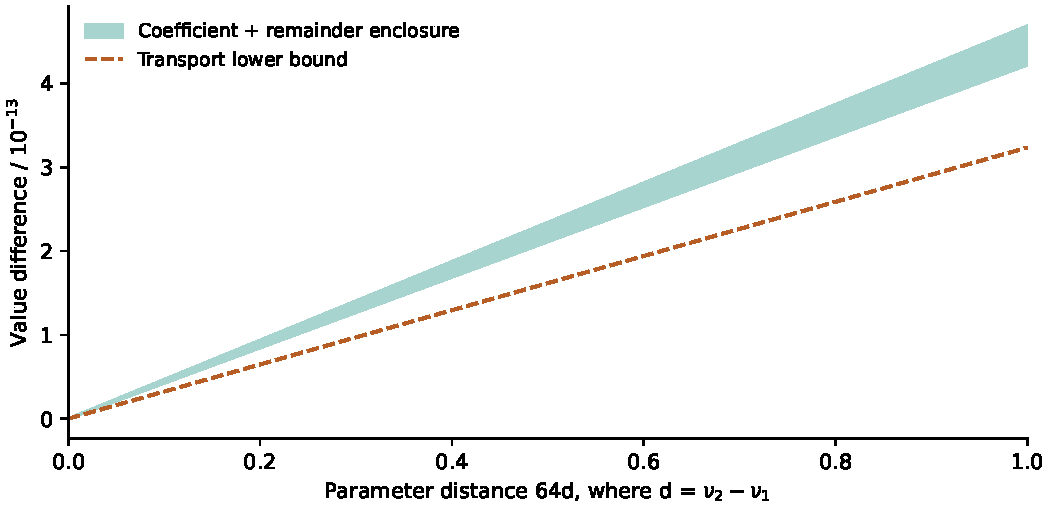
\includegraphics[width=.86\linewidth]{figures/theta_comparison.pdf}
 \caption{Guaranteed bounds on the change of the optimal value at
 \(M=2\cdot10^{-5}\), for any two driver parameters at distance \(d\).
 The shaded region is the coefficient-plus-remainder enclosure derived
 in this section.
 The dashed line is the weaker but strictly positive transport bound
 \(2.07\cdot10^{-11}d\). This plot displays bounds, not numerically
 computed finite-budget optimizers. At \(d=0\) the exact difference is zero.}
\end{figure}


\section{Scope, reproducibility, and questions for review}\label{sec:scope}
The resulting picture is that smoothing a sign-optimal moment design has
a computable leading amplitude cost and a fourth-order correction which
records the coupling to the lower moments. In the theta example, this
description is effective at stated budgets, and the least required amplitude
increases along the chosen cusp parameter interval. This is the concrete
optimization conclusion of the paper.

The finite-switch result identifies a unique optimizing profile for sufficiently
large \(M\). The countably infinite result identifies the value asymptotics and
proves attainment; it does not establish uniqueness or differentiability of the
finite-\(M\) optimizer. The theta error bound is specific to
\(\nu\in[-1/64,0]\) and \(M\geq2\cdot10^{-5}\). It is not a uniform result
on the longer exploratory cusp arc.

The target \(f_\nu\), the kernels, and the optimizing profile all vary with
\(\nu\). Strict comparison concerns these explicitly defined, different
optimization problems. It is not a comparison with a common target or a common
profile. The expansion with an \(O(M^{-6})\) error does not identify a coefficient
of \(M^{-6}\). Nor does the paper prove monotonicity of a normalized fourth-order
remainder at arbitrarily close parameters.

The moment construction gives a zero of order at least four for the modified
integral at its prescribed point. Exactly fourth order, a nondegenerate
unfolding of the modified family, and global root counts require further
conditions. No conclusion about the Riemann hypothesis, a de Bruijn--Newman
constant, a physical system, or an AI training procedure is drawn.

The accompanying source and evidence index identify which claims are analytic,
which use outward interval bounds, and which numerical plots are diagnostic.
An interval certificate is a finite collection of enclosures used with stated
analytic arguments; it is not a certification of the manuscript as a whole.
The checks can expose inconsistencies and reproduce enclosures, but are not a
machine-checked proof of the analytic arguments.

The main requests to an independent reviewer are: the weighted Taylor
interchanges and finite moment repair in Theorem~\ref{thm:infinite}; the
effective primal and dual estimates behind Theorem~\ref{thm:theta}; and the
characteristic inequality used in Theorem~\ref{thm:transport}. Questions of
novelty relative to bounded Lipschitz optimization are also open to review.

\paragraph{Use of AI-assisted tools.}
AI assistants were used in exploratory calculations, code development, proof
drafting, and internal checking. Exact algebra and interval computations are
reported separately from those assistants' assessments. Independent expert
review is being sought. The author is responsible for the submitted claims.

\appendix
\section{Effective support bounds and exact feasibility}\label{app:effective}
This appendix records the analytic estimates used by the finite interval
calculations. All constants below are evaluated on whole parameter and root
boxes. Point evaluations at approximate roots do not suffice.

\subsection{Local estimates}
Put \(a_0=2^{-14}\), \(\epsilon=2^{-12}\) and
\(b(a)=b^*+va^2\). At an original residual zero \(z_k\), start with the
center \(c_k=z_k+\kappa_ka^2\), with \(\kappa_k\) from \eqref{eq:kappa}.
Write \(K=|\kappa_k|\),
\(Q_{j,\ell,k}=\sup_{N_k}|q_j^{(\ell)}|\), and
\(R_{\ell,k}=\sup_{N_k}|q_*^{(\ell)}|\).
In the following formulas, unlabelled derivatives are evaluated at \(z_k\).
The moment change at this switch is exactly
\[
 \Delta_{j,k}=-2\sigma_k\mathbb E
                 \int_0^{\kappa_ka^2+ay}q_j(z_k+x)\dd x .
\]
Taylor's formula gives
\[
 |\Delta_{j,k}-a^2(-2\sigma_kq_j\kappa_k-\sigma_kq_j'/3)|
                  \leq H_{j,k}a^4 ,
\]
where
\begin{align*}
 H_{j,k}={}&|q_j'|K^2
 +\frac{|q_j''|}{3}(K+K^3a_0^2)\\
 &+\frac{Q_{j,3,k}}{12}(1/5+2K^2a_0^2+K^4a_0^4).
\end{align*}
For the residual, whose value at its zero is exactly zero,
\[
 \Delta_{*,k}=-\sigma_kr_ka^2/3
 -\sigma_k(r_k\kappa_k^2+t_k\kappa_k/3+u_k/60)a^4+\varepsilon_k,
 \qquad |\varepsilon_k|\leq K_{*,k}a^6,
\]
with
\begin{align*}
 K_{*,k}={}&|t_k|K^3/3+|u_k|(2K^2+K^4a_0^2)/12\\
 &+|q_*^{(4)}|(K+(10/3)K^3a_0^2+K^5a_0^4)/60\\
 &+R_{5,k}(1/7+3K^2a_0^2+5K^4a_0^4+K^6a_0^6)/360 .
\end{align*}
These coefficients come from signed averages of powers, including
\(\mathbb E(\kappa a^2+ay)^5=\kappa a^6+(10/3)\kappa^3a^8+\kappa^5a^{10}\).
Bounding that odd average by an absolute fifth moment would lose the
required order.

For \(F_k(c)=\mathbb E q_{b(a)}(c+ay)\), the quadratic coefficient at
\(c_k\) vanishes because \(r_k\kappa_k+t_k/6-Q_k^{\mathsf T}v=0\).
Thus \(|F_k(c_k)|\leq h_ka^4\), where
\begin{align*}
 h_k={}&|t_k|K^2/2+|u_k|(K+K^3a_0^2)/6\\
 &+R_{4,k}(1/5+2K^2a_0^2+K^4a_0^4)/24\\
 &+\sum_{j<3}|v_j|\{
       |q_j'|K+Q_{j,2,k}(1/3+K^2a_0^2)/2\}.
\end{align*}
If the signed derivative \(\sigma_kF_k'\geq m_k>0\) on the relevant
center interval, the true balanced center is within \(h_ka^4/m_k\).
The local objective has second derivative at most \(-2m_k\).
Its possible increase after balancing is consequently at most
\(h_k^2a^8/m_k\). Containment of both ramps is checked before this
estimate is applied.

Move the first three centers by \(a^4y_k\), with
\(|y_k|\leq W_k\), \(W=(2^{26},2^{26},2^{24})\).
For \(J_{jk}=-2\sigma_kq_j(z_k)\), let \(C\) be the dyadic
preconditioner recorded for the cell. The Jacobian deviation is bounded by
\[
 \Delta J_{jk}\leq
 2\{Q_{j,1,k}(K_ka_0^2+W_ka_0^4)+Q_{j,2,k}a_0^2/6\}.
\]
In the norm \(\max|y_k|/W_k\), the map subtracting \(C\) times the
lower moments divided by \(a^4\) has the following uniform bounds:
\[
 \text{derivative rows}<(.005731,.007842,.004703),\qquad
 \text{forcing}<(.328781,.448496,.267009).
\]
Each corresponding sum is less than one. The contraction theorem gives
exactly vanishing lower moments within this center construction.
The same estimates imply that \(C\) is nonsingular.
With \(\mathcal L_k=\sup|q_{b(a)}'|\), the repair costs at most
\[
 a^8\sum_{k=1}^3(2h_kW_k+\mathcal L_kW_k^2).
\]
This estimate is made for \(q_{b(a)}\), whose center derivative is of
order \(a^4\). The repaired target equals its \(q_3\) target because
the lower moments vanish.

\subsection{A changing finite prefix and its entire omitted tail}
Always retain the 28 zeros below \(1\). Retain a tail zero \(z_k>1\)
precisely when \(ae^{4z_k}\leq\epsilon\).
This gives a finite prefix for every \(a>0\).
After the last active ramp, extend its final plateau to infinity.
The first inactive zero is separated from the finite interval by the
validated positive gap \([1,1.001]\).

Uniformly on the driver cells, \(|v|<(5,4,180)\) and the expanded
trial multiplier box satisfies
\(|b|<(.001,.1,.005)\).
On each active tail neighborhood \([z_k-3a,z_k+3a]\), the raw phase
estimates give \(|\kappa_k|<46e^{4z_k}\), signed raw trial derivative
greater than \(550z_k^3\), and raw absolute value less than \(2800az_k^3\).
Also \(\tfrac12<w(x)/w(z_k)<2\), since the logarithmic variation
is less than \(408\epsilon<1/2\).
Combining the weight derivative with these estimates gives
\(\sigma_k q_{b(a)}'>200w(z_k)z_k^3\).
Thus balancing is valid on active tail neighborhoods as well.

For \(u\geq1\), the weight satisfies
\[
 w_\nu(u)\leq88e^{9u+9u^4-\pi e^{4u}} .
\]
Writing \(P_\nu=\lambda u^2+\mu u^4+\nu u^6\) and \(H=1/64\),
\begin{align*}
 |P_\nu'|&\leq44u^3+6Hu^5,&
 |P_\nu''|&\leq116u^2+30Hu^4,\\
 |P_\nu'''|&\leq216u+120Hu^3,&
 |P_\nu^{(4)}|&\leq216+360Hu^2,&
 |P_\nu^{(5)}|&\leq720Hu .
\end{align*}
The inequalities \(e^{4u}>50u^3\) and \(u^5e^{-4u}<1/40\) imply
\(|P_\nu^{(j)}|<e^{4ju}\), \(1\leq j\leq5\).
The theta derivatives follow from
\[
 P_0(x)=-3+2x,\qquad
 P_{\ell+1}(x)=(5-4x)P_\ell(x)+4xP_\ell'(x),
\]
applied term by term to \(\Phi\); product rules and exponential
derivative polynomials give the needed five weight derivatives.
This retains the sextic terms in local calculations and discards
their negative exponent only when taking an upper tail bound.

For \(0\leq p\leq3\), \(d\in\{12,16,24\}\), the corresponding root
sum and integral are bounded by
\[
 S_d=\frac{88e^{18+d-\pi e^4}}{1-50^{-4}},\qquad
 I_d=\frac{88}{500}e^{18+d-\pi e^4}.
\]
Indeed the logarithmic derivative of the envelope is below \(-500\);
root spacing exceeds \(3/85\), giving a successive term ratio below
\(50^{-4}\).
For every nonnegative sequence \(t_k\), inactive roots satisfy
\[
 \sum_{ae^{4z_k}>\epsilon}t_k
       \leq(a/\epsilon)^s\sum_k t_ke^{4sz_k}\quad(s>0).
\]
This supplies the missing powers of \(a\); a fixed cutoff would not.
For example the inactive quadratic and fourth coefficients are paid for
by \(300\epsilon^{-4}S_{16}\) and
\(2071000\epsilon^{-2}S_{16}\), respectively, at sixth order.
The lower-moment coefficient uses \(188\epsilon^{-2}S_{12}\).
Cutting the final integral at the first inactive zero minus \(3a\)
gives the additional bounds
\[
 \frac{18\epsilon^{-6}I_{24}}{1-72a_0},\qquad
 \frac{2^{j+1}\epsilon^{-4}I_{16}}{1-48a_0}
\]
for the normalized objective and lower-moment tails.
Active tail derivatives use the same envelope with the local formulas
above. The evidence records these sums, signs, and containment margins.

Combining the finite part, the active tail, and the inactive tail yields,
for every fixed \((\nu,a)\in I\times(0,a_0]\),
\begin{align}
 H_{b(a)}(a)&\leq D-\Gamma a^2/3+\Xi a^4+K_da^6,\label{eq:effectivesupport}\\
 |S(a)-(D-\Gamma a^2/3+\Xi a^4)|&\leq K_pa^6,\label{eq:effectiveprimal}
\end{align}
where \(K_d<655000\) and \(K_p<4.746\cdot10^6\) suffice uniformly.
During each three-center contraction, \(a\) and hence the prefix are
fixed. Continuity of the prefix as a function of \(a\) is not used.

\subsection{Scalar feasibility and inversion}
Set \(U=9.181\cdot10^{-10}\) and define
\[
 F_M(A)=DA-\Gamma A^3/(3M^2)+\Xi A^5/M^4,\qquad
 J_M(A)=F_M(A)-K_pA^7/M^6.
\]
On every driver cell, interval evaluation proves, for all \(M\geq M_0\),
\[
 J_M(\delta_0)<f<J_M(U),\qquad J_M'>0\text{ on }[\delta_0,U],
 \qquad U/M_0<a_0.
\]
The upper endpoint's normalized margin exceeds \(1.7683\cdot10^{-15}\).
Let \(A_+\) be the scalar root \(J_M(A_+)=f\).
At \(a=A_+/M\), \eqref{eq:effectiveprimal} gives \(S(a)\geq f/A_+\).
Multiplication of the repaired profile by \(A=f/S(a)\leq A_+\)
gives exact target and slope \(A/a\leq M\). This proves feasibility
at every budget despite changes in the prefix. Attainment follows as
in Theorem~\ref{thm:infinite}.

For the optimizer, \eqref{eq:effectivesupport} gives
\(F_M(\delta(M))\geq f-K_dU^7/M^6\).
The scalar upper root gives the corresponding upper comparison.
To bound the residual of \(P_4\), put
\[
 w=(\delta_0/M)^2,\quad t=\Gamma/(3D),\quad e=\Xi/D,\quad
 p=1+tw+(3t^2-e)w^2 .
\]
Then \(F_M(P_4)/f-1=p-twp^3+ew^2p^5-1\).
This is a polynomial of degree twelve whose coefficients through
degree two vanish exactly. Bounding all remaining coefficients on
\(0\leq w\leq(\delta_0/M_0)^2\) gives
\(|F_M(P_4)-f|\leq K_{\rm poly}/M^6\).
Also \(P_4\in[\delta_0,U]\) and
\[
 F_M'\geq d_{\min}=D_{\rm lo}-\Gamma_{\rm hi}U^2/M_0^2>0 .
\]
The inverse comparison constants are
\[
 K_-=\frac{K_{\rm poly}+K_dU^7}{d_{\min}}<1.001\cdot10^{-53},
 \qquad
 K_+=\frac{K_{\rm poly}+K_pU^7}{d_{\min}}<1.620\cdot10^{-53}.
\]
Rounding these bounds outwards gives \eqref{eq:thetaerror}.

\section{Verifying the transport condition on an unbounded domain}
\label{app:transport}
The uniform caps used here are
\[
 \lambda\in(-3.651,-3.645),\quad\mu\in(8.330,8.336),\quad
 \nu\in[-1/64,0],
\]
together with the derivative caps in the proof of
Corollary~\ref{cor:thetaorder}. For \(\Phi=\sum\phi_n\), put
\(x=\pi e^{4u}\) and, for \(n\geq2\),
\[
 R_n=\frac{\phi_n}{\phi_1}
 =n^2\frac{2n^2x-3}{2x-3}e^{-(n^2-1)x},\qquad
 \ell_n=9+\frac{12}{2n^2x-3}-4n^2x.
\]
Then \(\ell_n'=-16n^2x-96n^2x/(2n^2x-3)^2\).
For \(R=\sum_{n\geq2}R_n\),
\begin{equation}\label{eq:logtheta}
 L_\Phi=\ell_1+\frac{R'}{1+R},\qquad
 L_\Phi'=\ell_1'+\frac{R''}{1+R}
                      -\left(\frac{R'}{1+R}\right)^2 .
\end{equation}
On \(x\geq3\),
\[
 R_n\leq2n^4e^{-(n^2-1)x},\quad
 |R_n'|\leq10n^6xe^{-(n^2-1)x},\quad
 |R_n''|\leq100n^8x^2e^{-(n^2-1)x}.
\]
These follow by differentiating the displayed ratio; its logarithmic
derivative has absolute value at most \(5n^2x\), and the difference
of the logarithmic second derivatives has absolute value at most
\(20n^2x\). The summable majorants also justify the differentiations.

For \(0\leq u\leq1\), include \(n=2,\ldots,12\) explicitly.
The remaining errors in \(R,R',R''\) are bounded by
\[
 4\cdot13^4e^{-504},\quad60\cdot13^6e^{-504},\quad
 1800\cdot13^8e^{-504},
\]
because consecutive majorants have ratio below \(1/2\).
Arb evaluation of \eqref{eq:logtheta} on each of the 1024 whole
intervals \([i/1024,(i+1)/1024]\), using all parameter caps simultaneously,
then bounds
\begin{align*}
 L_\nu&=L_\Phi+2\lambda u+4\mu u^3+6\nu u^5,\\
 r&=-f'/f+4\kappa+\lambda'u^2+\mu'u^4+u^6+\kappa uL_\nu,\\
 r_u&=2\lambda'u+4\mu'u^3+6u^5+\kappa(L_\nu+uL_\nu').
\end{align*}
The largest recorded upper endpoint of \(r+\kappa+a_0|r_u|\) is
less than \(-0.02170697\); a separate outward rational reconstruction
proves the simpler bound \(<-0.0217<-1/50\) on every cell.

For \(u\geq1\), \(x>150\) and
\[
 R<64e^{-450},\quad |R'|<192000e^{-450},\quad
 |R''|<1152000000e^{-450}.
\]
Each is less than \(1/4\), and \(R'<0\). Equation~\eqref{eq:logtheta}
therefore gives
\[
 L_\Phi\leq10-4x,\quad |L_\Phi|\leq4x+1,\quad
 |L_\Phi'|\leq16x+2.
\]
For \(H=1/64\),
\begin{align*}
 L_\nu&\leq10-4x+36u^3<0,\\
 |L_\nu|&\leq4x+1+8u+36u^3+6Hu^5,\\
 |L_\nu'|&\leq16x+10+108u^2+30Hu^4 .
\end{align*}
Set \(k_-=.00259\), \(k_+=.00260\), \(l=.3264\),
\(m=.2942\), \(F=.0437\), and \(\bar k=k_--5a_0k_+>0\).
Using the sign of \(L_\nu\) in the term without absolute values,
\[
 r+\kappa+a_0|r_u|\leq P_6(u)-4\bar k\pi u e^{4u}=:Q(u),
\]
where, in increasing degree, the coefficients of \(P_6\) are
\[
 \begin{gathered}
 -F+5k_++a_0k_+,\quad 10k_-+a_0(2l+18k_+),\quad l,\\
 a_0(4m+144k_+),\quad m+36k_-,\quad
 a_0(6+36Hk_+),\quad1 .
 \end{gathered}
\]
All positive-degree coefficients are positive.
With \(S=\sum_{j=1}^6jP_j\), \(P_6'(u)\leq Su^5\).
The inequality \((1+4u)e^{4u}>270u^5\) for \(u\geq1\)
follows on writing \(z=u-1\), using \(e^4>109/2\) and the first six
Taylor terms for \(e^{4z}\). The difference polynomial has initial
coefficients \(5/2,-42,352\), forming a positive quadratic, and all
higher coefficients positive. Exact rational arithmetic then gives
\begin{align*}
 Q'(u)&<(S-4\bar k\cdot3\cdot270)u^5<0,\\
 Q(1)&<\sum P_j-4\bar k\cdot170\\
     &=-0.051116612396240234375<-1/50 .
\end{align*}
This proves the required inequality on the entire tail.

\section{Evidence, branch identification, and replay}\label{app:evidence}
The supplement preserves the numbered research packages as a fixed snapshot.
Their identifiers describe provenance, not additional unpublished theorems
which a reader must accept without a proof. The analytic arguments used
in this paper are given above; detailed local numerical witnesses and
coefficient differentiation formulas are in the indicated files.

\begin{center}\small
\begin{tabular}{p{.20\linewidth}p{.18\linewidth}p{.52\linewidth}}
\toprule
Claim & Evidence packages & Principal material\\
\midrule
General expansion & R21--R23 &
Finite and countable-switch proofs, exact algebra, examples\\
Cusp identity & R01, R03, R09, R29 &
Integral root box, connected uniqueness tubes, positive majorants,
32 driver cells\\
Theta coefficients & R24, R28, R29 &
Full root sums, weighted tails, implicit differentiation\\
Effective remainder & R25--R27, R30 &
Local jets, finite repair, moving prefix, scalar inversion\\
Actual-value order & R31 &
Moment identity, 1024 spatial cells, whole-tail comparison\\
\bottomrule
\end{tabular}
\end{center}

For reproducibility, the supplement includes the source, data, and dependency
closure of these packages. Its index maps each identifier to a directory,
manifest, proof, producer, and checker.
The following commands use paths relative to the supplement root:
\begin{verbatim}
python -B research/finite_slope_optimum/audit_snapshot.py
python -B research/finite_slope_fourth_order/audit_snapshot.py
python -B research/infinite_slope_fourth_order/audit_snapshot.py --with-arb
python -B research/cusp_order_transport/audit_snapshot.py --with-arb
\end{verbatim}
The last command recursively checks the later theta dependencies.
It regenerates the 1024 spatial interval enclosures, reconstructs the
32 driver-cell chain, and checks arithmetic and recorded prerequisites.
The accompanying report distinguishes freshly evaluated transcendental
enclosures from frozen prerequisite inputs.
The implementation uses Python, python-flint/Arb \cite{arb,integration},
exact rational arithmetic, and mpmath for non-rigorous diagnostics.
Pinned versions and input hashes are supplied.

Some details concerning identity and differentiation deserve emphasis.
The initial cusp is enclosed by an integral-based contraction, with
\(D_3D_4\ne0\). In the original continuation, the scaled contraction
bound is below \(0.502\) and the forcing-plus-contraction bound
is below \(0.560\).
At adjacent faces a smaller root enclosure lies inside the next full
uniqueness box. On the short interval used here, refined anchors and
degree-five parameter expansions with sixth-order remainder remain
inside those already identified tubes.
Thus a collection of unrelated zeros is not substituted for a branch.

The lower sign-moment equations have derivative \(-G\).
Their implicit solution \(b^*(\nu)\), and the simple residual zeros,
are differentiated together. For example,
\[
 \delta_0'=(f'D-fD')/D^2,\qquad
 C_2'=C_2(3f'/f-4D'/D+\Gamma'/\Gamma).
\]
The \(b^{*\,\prime}\) contribution to \(D'\) vanishes by the sign
moments; it does not vanish from \(\Gamma'\).
Root-sum derivatives retain root motion. Their tail bounds are justified
by separated zeros, implicit derivative bounds, and double exponential
majorants of the same type as \eqref{eq:weighted}.
The package R29 gives the termwise formulas and enclosing intervals
used for \eqref{eq:coefficientmotion}.

The final transport audit records 31 exact algebra groups,
19,017 rational decisions, and 1024 closed spatial cells. Its independent
high-precision integral and composition diagnostics are useful consistency
checks, but are not interval proofs.
The rational checker uses stated transcendental enclosures as inputs;
it is not a second independent rigorous integration engine.
The four replay entry points passed on 23 September 2026, and
1,334 entries in 32 pre-existing manifests remained unchanged.
These counts establish the tested snapshot and the coverage of that
replay. They do not establish that every line of analytic reasoning
is error-free.

For the public supplement, local machine paths in bookkeeping records are
replaced by neutral placeholders. All dependent checksum references are
updated consistently, and the complete transformation map is supplied.
No mathematical formula or numerical enclosure is changed by that
transformation. The public copy is replayed separately; its manifest
identities are therefore distinguished from the original local snapshot.

\clearpage
\begin{thebibliography}{9}
\bibitem{lellmann}
J.~Lellmann, D.~A. Lorenz, C.~Sch\"onlieb, and T.~Valkonen,
\emph{Imaging with Kantorovich--Rubinstein discrepancy},
SIAM Journal on Imaging Sciences 7 (2014), 2833--2859.
\href{https://doi.org/10.1137/140975528}{doi:10.1137/140975528}.
Preprint: \url{https://arxiv.org/abs/1407.0221}.

\bibitem{hille2023}
S.~C. Hille and E.~S. Theewis,
\emph{Explicit expressions and computational methods for the
Fortet--Mourier distance of positive measures to finite weighted sums of
Dirac measures}, Journal of Approximation Theory 294 (2023), 105947.
Preprint:
\url{https://arxiv.org/abs/2206.12234}.

\bibitem{hille2024}
S.~C. Hille and E.~S. Theewis,
\emph{Norming and dense sets of extreme points of the unit ball in
spaces of bounded Lipschitz functions},
Journal of Mathematical Analysis and Applications 536 (2024), 128200.
Preprint:
\url{https://arxiv.org/abs/2305.08500}.

\bibitem{abbar}
A.~Abbar, C.~Coine, and C.~Petitjean,
\emph{A pre-adjoint approach on weighted composition operators between
spaces of Lipschitz functions}, preprint, 2023.
\url{https://arxiv.org/abs/2304.12173}.

\bibitem{lessard}
J.-P. Lessard and A.~Pugliese,
\emph{Cusp bifurcations: numerical detection via two-parameter
continuation and computer-assisted proofs of existence},
Linear Algebra and its Applications 728 (2026), 26--46.
\href{https://doi.org/10.1016/j.laa.2025.08.015}{doi:10.1016/j.laa.2025.08.015}.
Preprint: \url{https://arxiv.org/abs/2404.00535}.

\bibitem{arb}
F.~Johansson,
\emph{Arb: Efficient arbitrary-precision midpoint-radius interval arithmetic},
preprint, 2016.
\url{https://arxiv.org/abs/1611.02831}.

\bibitem{integration}
F.~Johansson,
\emph{Numerical integration in arbitrary-precision ball arithmetic},
preprint, 2018.
\url{https://arxiv.org/abs/1802.07942}.
\end{thebibliography}

